\chapter{Redes Neuronales y Deep Learning}
\label{chapter:redes-neuronales-deep-learning}

En este capítulo vamos a dar un repaso a la teoría básica de Redes Neuronales y Deep Learning antes de entrar en la práctica. Repasaremos los fundamentos del aprendizaje con Redes Neuronales, veremos las estructuras de Aprendizaje Profundo o Deep Learning así como las capas de dichas redes que emplearemos en la práctica. Por último veremos una estructura de red que será utilizada en algunos de los modelos, los Autoencoders.

Para la elaboración de este capítulo nos basaremos en los libros de Bengio \cite{goodfellow_deep_2016} y Zaccone \cite{giancarlo_deep_2017}.

\section{Aprendizaje de las Redes Neuronales}

No todas las redes que vamos a emplear en la parte práctica corresponden al modelo ``Feedforward'', ya que también vamos a elaborar redes neuronales con capas recurrentes, pero vamos a estudiar el comportamiento primero de estas redes para luego explicar las modificaciones que dichas arquitecturas añaden.

En primer lugar, llamamos a este tipo de redes prealimentadas o ``Feedforward'' en inglés, porque la información fluye siempre en un sentido, desde la entrada hasta la salida obtenida. En las redes denominadas como recurrentes este sentido de la información se revierte en algunos puntos, realimentando la red con la propia salida de algunas capas o de todas ellas.

La representación más común de una red neuronal profunda es a través de la composición de funciones. Supongamos que estamos aproximando la función $f*(x)$ con una función $f(x)$ construida mediante tres funciones distintas: $f^{(1)}, f^{(2)} \ y \ f^{(3)}$ en este mismo orden. Entonces la representación de la función $f$ quedaría como:

$$f(x) = f^{(3)}(f^{(2)}(f^{(1)}(x))),$$

donde $x$ es la entrada de la red neuronal o lo que es lo mismo, una instancia o varias de nuestro conjunto de datos. En este caso además decimos que $f^{(1)}$ es la primera capa de la red, $f^{(2)}$ la segunda capa, etcétera.

Este tipo de estructuras se llaman profundas al tener varias capas y por tanto varias funciones que, al componerlas, aproximarán la función objetivo que tenemos. Las capas que se encuentran entre la primera y la última, al no ser capas ``visibles'' desde el exterior de la red las denominamos capas ocultas.

Estas capas están compuestas de unidades que denominamos neuronas haciendo una equivalencia con el modelo biológico. Una neurona recibe un número de entradas fijado, por ejemplo $n$. Para cada una de las entradas que recibe va aprendiendo un peso $w$, que luego multiplicará a cada una de las entradas y sumará para obtener un valor ponderado. A este valor ponderado se le aplica una función de activación que nos convierte dicho valor al rango que nosotros queramos para nuestro problema. Por tanto, una neurona produce como salida la función de activación aplicada a una combinación lineal de las entradas que recibe.

\begin{figure}[H]
	\centering
	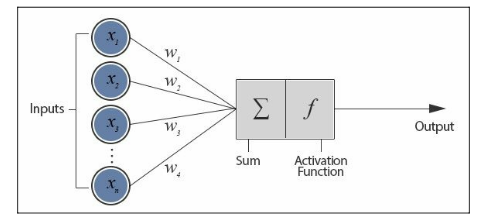
\includegraphics[scale=0.65]{imagenes/neurona.png}
	\caption{Representación de una neurona en una Red Neuronal.}
	\label{img:neurona}
\end{figure}

Como un detalle más a tener en cuenta, solemos añadir a las entradas una que denominamos como sesgo. Este sesgo es 1 y se suma a la combinación lineal, haciendo de término independiente en la ecuación de la recta que se está representando en el espacio de dominio de las instancias.

En cuanto a funciones de activación tenemos muchas sobre las que escoger, veamos las más comunes:

\begin{itemize}
	\item Rectified Linear Unit (ReLU): esta función de activación se define como 
	$$ReLU(x) = x^+ = max(0,x) \ , \ x\in \mathbb{R}^d,$$
	es decir, cero en los negativos y la función identidad en los positivos.
	\begin{figure}[H]
		\centering
		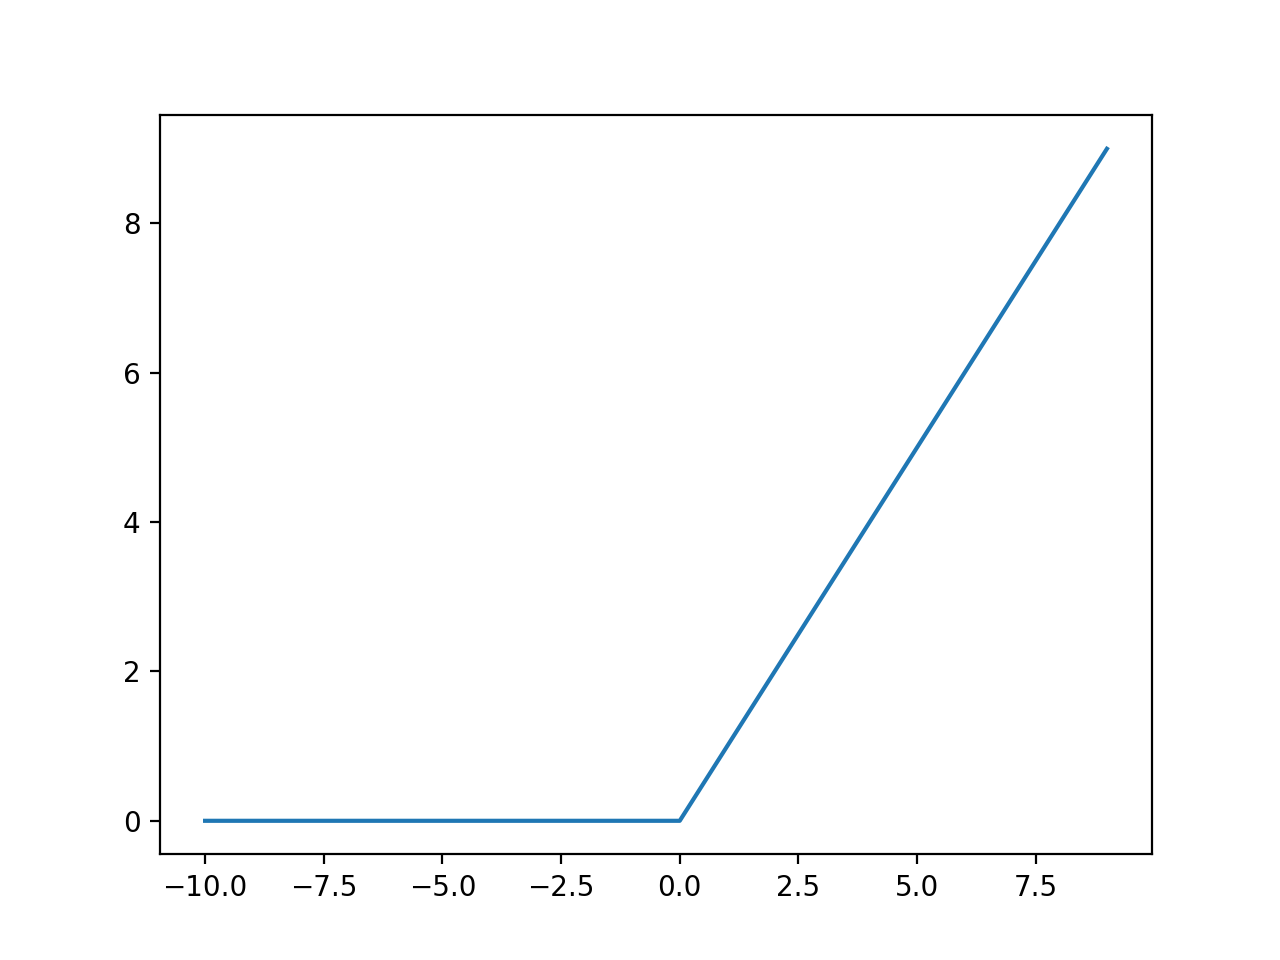
\includegraphics[scale=0.5]{imagenes/relu.png}
		\caption{Función ReLU.}
		\label{img:relu}
	\end{figure}
	\item Softmax: esta función de activación se define como:
	$$softmax : \mathbb{R}^d \rightarrow [0,1]^d$$
	$$softmax(x)_j = \frac{e^{x_j}}{\sum_{k=1}^{d}e^{x_k}}$$
	Con esta función se obtiene un valor con el mismo número de dimensiones que el que tuvieran los datos de entrada. Además, la salida se puede emplear para representar una distribución de probabilidad. Normalmente esta función de salida se emplea en problemas de clasificación donde vamos a obtener un valor entre 0 y 1 para cada una de las clases, siendo el mayor de estos la clase que el modelo predice.
	\item Sigmoide: esta función de activación se define como:
	$$sigmoide(x) = \frac{1}{1+e^{-x}}$$
	Esta función es una función real de variable real muy conocida y estudiada en matemáticas, con propiedades interesantes como que posee dos asíntotas horizontales y tiene una primera derivada no negativa.
	\begin{figure}[H]
		\centering
		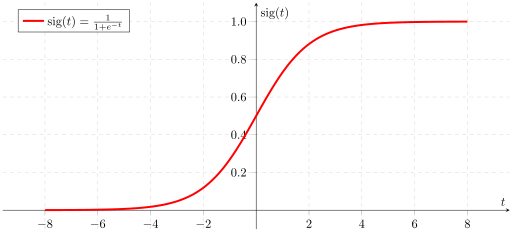
\includegraphics[scale=0.5]{imagenes/sigmoide.png}
		\caption{Función Sigmoide.}
		\label{img:sigmoide}
	\end{figure}
	Su valor máximo es $1$ y su valor mínimo es $0$.
	\item Tangente hiperbólica: la función tangente hiperbólica se define como:
	$$tanh : \mathbb{R}\rightarrow \mathbb{R} \ , \ tanh(x) = \frac{sinh(x)}{cosh(x)} = \frac{e^x - e^{-x}}{e^x + e^{-x}}$$
	\begin{figure}[H]
		\centering
		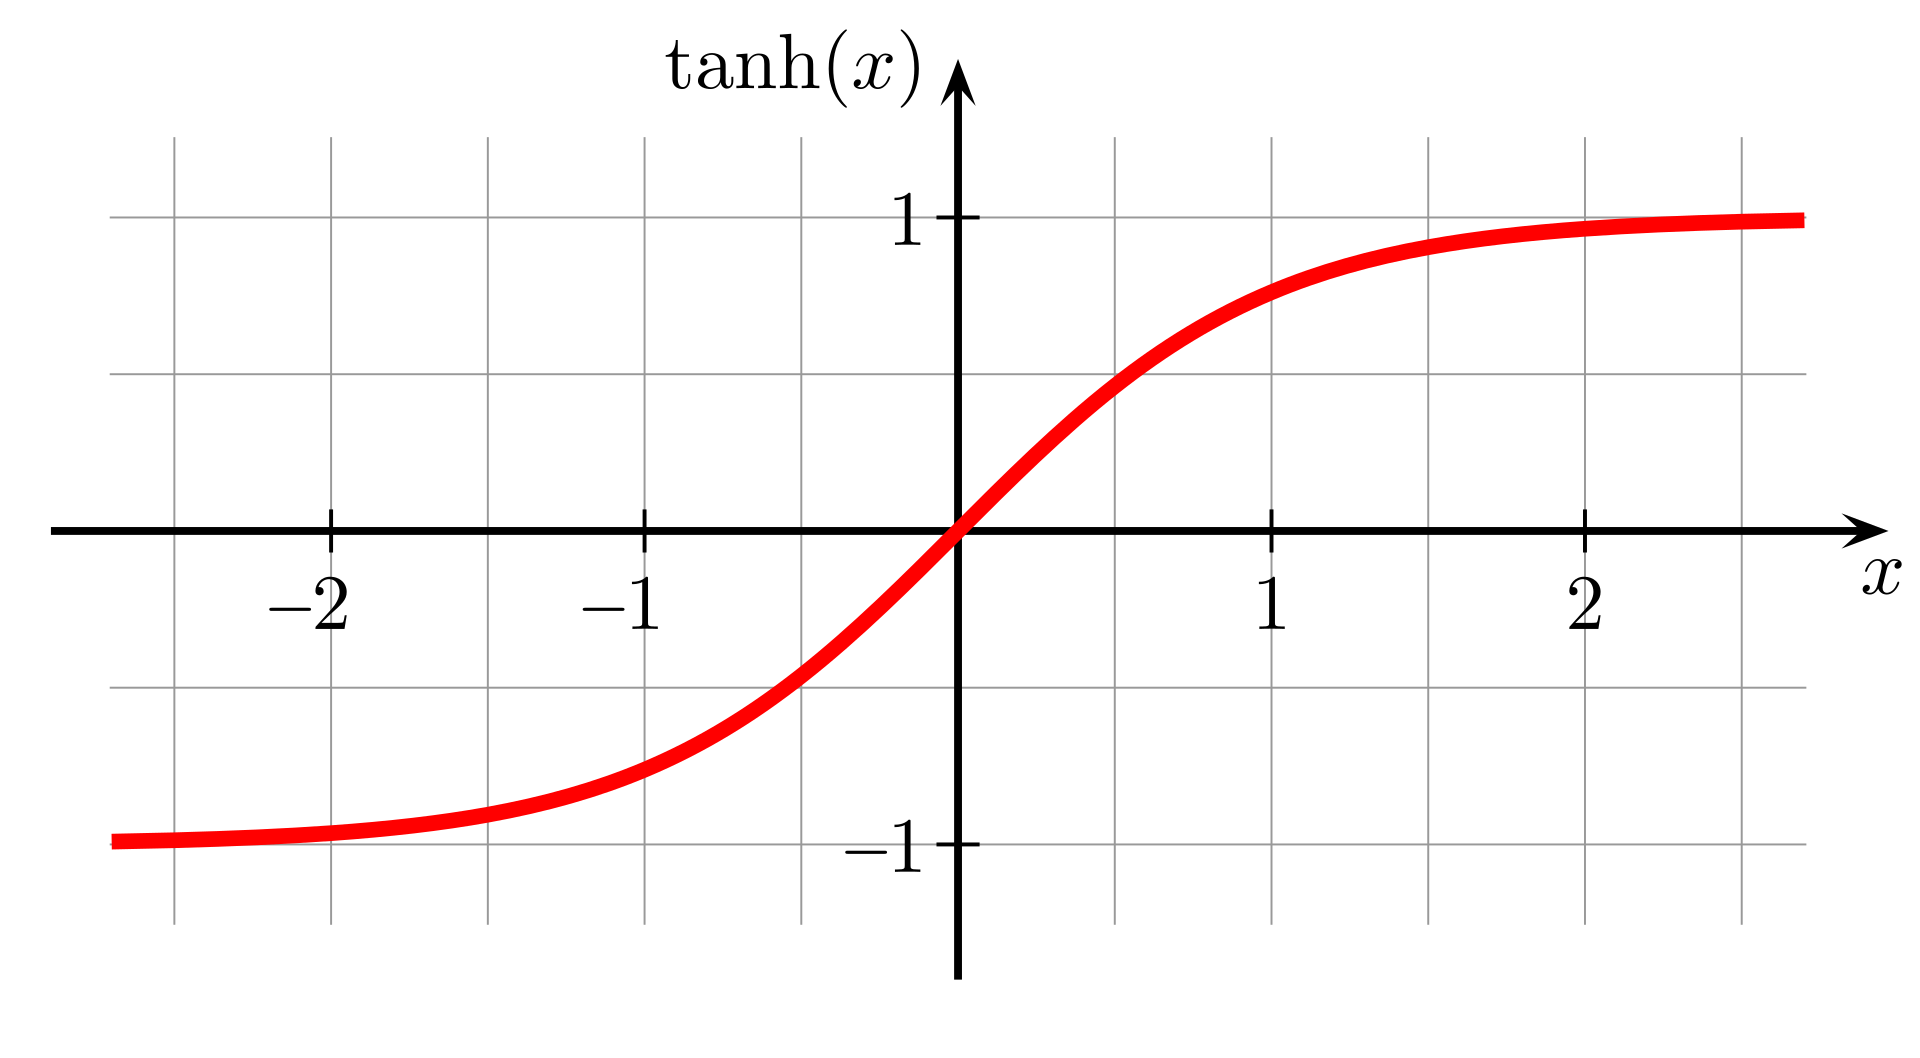
\includegraphics[scale=0.15]{imagenes/tangente_hiperbolica.png}
		\caption{Función tangente hiperbólica.}
		\label{img:tanh}
	\end{figure}
	Como podemos ver esta función de activación puede tomar valores en el intervalo $(-1,1)$.
\end{itemize}

Una vez que sabemos cuál es el comportamiento básico de una neurona vamos a ver cómo funciona el algoritmo empleado en el aprendizaje de las redes: Backpropagation.

Si describimos el proceso de forma sencilla podemos resumirlo en 4 pasos:

\begin{enumerate}
	\item Inicializar la red con pesos aleatorios.
	\item Calcular el error cometido en la predicción con los pesos actuales (pasada hacia delante) y, para cada una de las capas, ir volviendo hacia atrás desde la salida hasta la entrada.
	\item Enseñarle a la red el valor que debía predecir.
	\item Modificar los pesos en cada capa para mejorar la predicción.
\end{enumerate}

Lo primero que tenemos que hacer es definir las funciones de coste. Cuando estamos entrenando una red neuronal queremos tener una función de coste que optimizar, como hemos visto antes en la sección de Machine Learning. En este sentido podemos emplear varias funciones de coste en función de nuestras necesidades, pero es importante tener en cuenta que vamos a necesitar una para el proceso de aprendizaje.

En los cuatro pasos que hemos descrito, tras la inicialización de los pesos, tenemos el paso de la propagación hacia delante. Veamos este paso en pseudocódigo:

\begin{algorithm}[H]{\Large{\textbf{Propagación hacia delante}}}
	
	\vspace{15px}
	
	\caption{Propagación hacia delante}
	\label{alg:forward-propagation}
	\KwIn{Profundidad de la red $l$}
	\KwIn{Matriz de pesos para la capa i-ésima $W^{(i)}$}
	\KwIn{Vector de sesgos de la capa i-ésima $b^{(i)}$}
	\KwIn{Instancia a procesar $x$}
	\KwIn{Salida objetivo $y^*$}
	\KwIn{Función de activación $g$}
	\KwIn{Función de similitud $L$}
	\KwIn{Función de regularización $\Omega$}
	\KwIn{Parámetros del modelo $\theta$}
	\KwIn{Ponderación de la regularización $\lambda$}
	
	\vspace{10px}
	
	$h^{(0)}\leftarrow x$
	
	\For{$k=1,...,l$}{
		
		$z^{(k)}\leftarrow W^{(k)}h^{(k-1)} + b^{(k)}$
		
		$h^{(k)}\leftarrow g(z^{(k)})$
		
	}

	$y\leftarrow h^{(l)}$
	
	$J\leftarrow L(y,y^*) + \lambda \Omega (\theta)$
	
	\vspace{10px}
	
	\KwOut{Predicción hecha $y$}
	\KwOut{Error cometido $J$}
	
	\vspace{5px}
\end{algorithm}

Como podemos ver, este algoritmo se encarga de ir pasando la información desde la entrada (la propia instancia) por cada una de las capas, multiplicando por su peso correspondiente, sumando el sesgo y aplicando la función de activación hasta que obtenemos una salida final.

Hemos visto en las secciones de Machine Learning que, una forma de hacer que nuestros algoritmos aprendan, es necesario obtener el gradiente del error para poder avanzar en el aprendizaje. Para realizar esta labor tenemos el algoritmo Backpropagation, que nos ayudará a calcular dicho gradiente de forma eficiente. Pensemos que tenemos que calcular el gradiente del modelo derivando con respecto a todos los parámetros. Cuando hablamos de Deep Learning es común tener muchas capas ocultas con un número elevado de neuronas, lo que aumenta muchísimo el número de parámetros y por tanto la complejidad del cálculo del gradiente.

Vamos a poner un ejemplo para poder ver la complejidad del cálculo del gradiente:

\begin{figure}[H]
	\centering
	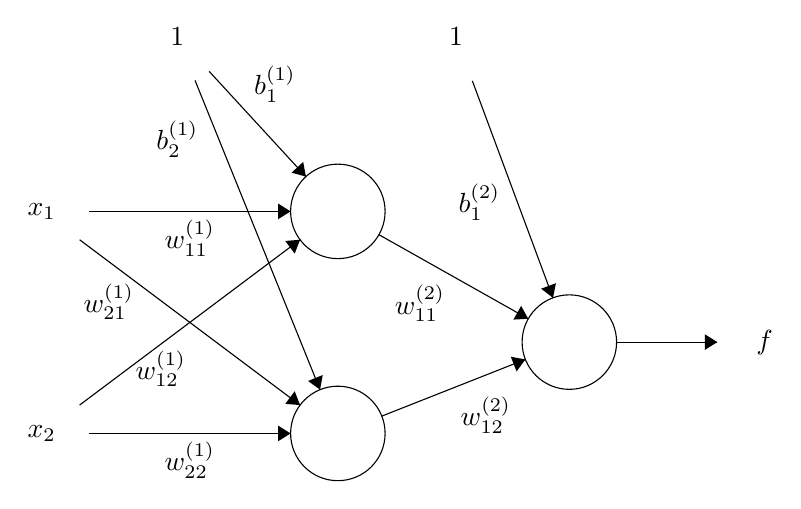
\begin{tikzpicture}[scale=0.2]
		\tikzstyle{every node}+=[inner sep=0pt]
		\draw [black] (34,-24.7) circle (3);
		\draw [black] (34,-38.8) circle (3);
		\draw [black] (48.7,-33) circle (3);
		\draw (15.2,-24.7) node {$x_1$};
		\draw (15.2,-38.8) node {$x_2$};
		\draw (61.1,-33) node {$f$};
		\draw (23.8,-13.6) node {$1$};
		\draw (41.5,-13.6) node {$1$};
		\draw [black] (36.79,-37.7) -- (45.91,-34.1);
		\fill [black] (45.91,-34.1) -- (44.98,-33.93) -- (45.35,-34.86);
		\draw (43.4,-36.44) node [below] {$w_{12}^{(2)}$};
		\draw [black] (36.61,-26.18) -- (46.09,-31.52);
		\fill [black] (46.09,-31.52) -- (45.64,-30.7) -- (45.15,-31.57);
		\draw (39.21,-29.35) node [below] {$w_{11}^{(2)}$};
		\draw [black] (17.6,-26.5) -- (31.6,-37);
		\fill [black] (31.6,-37) -- (31.26,-36.12) -- (30.66,-36.92);
		\draw (19.45,-29.25) node [below] {$w_{21}^{(1)}$};
		\draw [black] (17.6,-37) -- (31.6,-26.5);
		\fill [black] (31.6,-26.5) -- (30.66,-26.58) -- (31.26,-27.38);
		\draw (22.75,-33.50) node [below] {$w_{12}^{(1)}$};
		\draw [black] (51.7,-33) -- (58.1,-33);
		\fill [black] (58.1,-33) -- (57.3,-32.5) -- (57.3,-33.5);
		\draw [black] (25.83,-15.81) -- (31.97,-22.49);
		\fill [black] (31.97,-22.49) -- (31.8,-21.56) -- (31.06,-22.24);
		\draw (31.36,-16.61) node [left] {$b_1^{(1)}$};
		\draw [black] (42.54,-16.41) -- (47.66,-30.19);
		\fill [black] (47.66,-30.19) -- (47.85,-29.26) -- (46.91,-29.61);
		\draw (44.34,-24.11) node [left] {$b_1^{(2)}$};
		\draw [black] (24.93,-16.38) -- (32.87,-36.02);
		\fill [black] (32.87,-36.02) -- (33.04,-35.09) -- (32.11,-35.47);
		\draw (25.16,-20.1) node [left] {$b_2^{(1)}$};
		\draw [black] (18.2,-24.7) -- (31,-24.7);
		\fill [black] (31,-24.7) -- (30.2,-24.2) -- (30.2,-25.2);
		\draw (24.6,-25.2) node [below] {$w_{11}^{(1)}$};
		\draw [black] (18.2,-38.8) -- (31,-38.8);
		\fill [black] (31,-38.8) -- (30.2,-38.3) -- (30.2,-39.3);
		\draw (24.6,-39.3) node [below] {$w_{22}^{(1)}$};
	\end{tikzpicture}
	\label{fig:backpropagation-ejemplo}
	\caption{Ejemplo de una red neuronal sencilla.}
\end{figure}

Aquí podemos ver una red neuronal con 2 entradas y dos capas. Cada una de las capas tiene sus pesos y sus sesgos correspondientes. Entonces, en el modelo que hemos puesto como ejemplo, tenemos el siguiente vector de parámetros que determina nuestra red neuronal:

$$\theta = \Big(w_{11}^{(1)}, w_{12}^{(1)}, w_{21}^{(1)}, w_{22}^{(1)}, b_1^{(1)}, b_2^{(1)}, w_{11}^{(2)}, w_{12}^{(2)}, b_1^{(2)}\Big)$$

Con estos parámetros, la expresión de la salida de la red neuronal es:

$$f(x_1 , x_2 ; \theta) = g(w_{11}^{(2)}g(w_{11}^{(1)}x_1 + w_{12}^{(1)}x_2 + b_1^{(1)}) + w_{12}^{(2)}g(w_{21}^{(1)}x_1 + w_{22}^{(1)}x_2 + b_2^{(1)}) + b_1^{(2)})$$

Para simplificar las expresiones de las parciales vamos a notar lo siguiente:

$$\alpha = g' (w_{11}^{(2)}g(w_{11}^{(1)}x_1 + w_{12}^{(1)}x_2 + b_1^{(1)}) + w_{12}^{(2)} g(w_{21}^{(1)}x_1 + w_{22}^{(1)}x_2 + b_2^{(1)}) + b_1^{(2)}),$$

$$\beta =  g'(w_{11}^{(1)}x_1 + w_{12}^{(1)}x_2 + b_1^{(1)}) \ y$$

$$\gamma =  g'(w_{21}^{(1)}x_1 + w_{22}^{(1)}x_2 + b_2^{(1)}).$$

Con esto, podemos sacar las parciales de f, que nos van a ser necesarias en el cálculo del gradiente del coste J.

\footnotesize
\begin{alignat*}{3}
\frac{\partial f}{\partial w_{11}^{(1)}}(x_1,x_2;\theta)&=\alpha w_{11}^{(2)}\beta x_1,\quad&
\frac{\partial f}{\partial w_{12}^{(1)}}(x_1,x_2;\theta)&=\alpha w_{11}^{(2)}\beta x_2,\\
\frac{\partial f}{\partial w_{21}^{(1)}}(x_1,x_2;\theta)&=\alpha w_{12}^{(2)}\gamma x_1,\quad&
\frac{\partial f}{\partial w_{22}^{(1)}}(x_1,x_2;\theta)&=\alpha w_{12}^{(2)}\gamma x_2,\\
\frac{\partial f}{\partial b_{1}^{(1)}}(x_1,x_2;\theta)&=\alpha w_{11}^{(2)}\beta, \quad&
\frac{\partial f}{\partial b_{2}^{(1)}}(x_1,x_2;\theta)&=\alpha w_{12}^{(2)}\gamma, \\
\frac{\partial f}{\partial w_{11}^{(2)}}(x_1,x_2;\theta)&=\alpha g(w_{11}^{(1)}x_{1}+w_{12}^{(1)}x_2 + b_1^{(1)}),&&\\
\frac{\partial f}{\partial w_{12}^{(2)}}(x_1,x_2;\theta)&=\alpha g(w_{21}^{(1)}x_{1}+w_{22}^{(1)}x_2 + b_2^{(1)}),&\quad
\frac{\partial f}{\partial b_{1}^{(2)}}(x_1,x_2;\theta)&=\alpha.
\end{alignat*}
\normalsize

Viendo las expresiones que tenemos de las derivadas parciales se puede entender mejor la necesidad de eficiencia. En primer lugar, podemos ver que no tenemos una red para nada grande y ya tenemos que calcular 9 derivadas parciales. Por otro lado, podemos ver que hay términos que se repiten bastante con lo que, calculando primero estos términos, simplificamos la complejidad computacional de este problema.

Veamos el algoritmo de Backpropagation en pseudocódigo:

\begin{algorithm}[H]{\Large{\textbf{Propagación hacia atrás}}}
	
	\vspace{15px}
	
	\caption{Propagación hacia atrás}
	\label{alg:backpropagation}
	
	\vspace{10px}
	
	Calculamos el gradiente de la capa de salida.
	
	$d\leftarrow \nabla_y J(y,y^*;\theta) = \nabla_y L(y,y^*)$
	
	\For{$k=l,...,1$}{
	
		Aplicamos la regla de la cadena ($\odot$ es el producto componente a componente).
		
		$d\leftarrow \nabla_{z^{(k)}} J = d\odot g' (z^{(k)})$
		
		Calculamos los gradientes en los pesos y sesgos añadiendo también la regularización si la hubiera.
		
		$\nabla_{b^{(k)}}J = d + \lambda \nabla_{b^{(k)}} \Omega (\theta)$
		
		$\nabla_{W^{(k)}}J = d(h^{(k-1)})^T + \lambda \nabla_{W^{(k)}} \Omega (\theta)$
		
		$d\leftarrow \nabla_{h^(k-1)} J = \Big( W^{(k)} \Big)^T d$

	}
	
	\KwOut{Valor final del gradiente $d$}
	
	\vspace{5px}
\end{algorithm}

Como podemos ver, este algoritmo simplemente aplica la regla de la cadena y va calculando los gradientes sin repetir las derivadas capa a capa. Esta aproximación hace que el cálculo sea más sencillo y no se repita.

Llegados a este punto ya tenemos la salida que nos produce nuestra red neuronal con el algoritmo de propagación hacia delante y tenemos el cálculo del gradiente con la propagación hacia atrás. Ahora nos queda optimizar dicho coste con las herramientas que tenemos, es decir, resolver el problema de optimización que tenemos con el gradiente. 

Para resolver este problema tenemos la aproximación clásica de Gradiente Descendente Estocástico aunque no es la única herramienta que podemos usar para esto. Veremos algunas de las más utilizadas y cómo nos ayudan para obtener nuevos parámetros que mejoren el desempeño de las redes.

En primer lugar cabe explicar el algoritmo más empleado en esta tarea: Gradiente Descendente Estocástico. En Deep Learning se emplea el entrenamiento por lotes o batches en inglés, lo que hace inviable el uso de ténicas como Gradiente Descendente. Es por ello que se suele emplear la aproximación estocástica de Gradiente Descendente al ir calculando una aproximación del gradiente con números pequeños de muestras. Veamos el algoritmo en pseudocódigo:

\begin{algorithm}[H]{\Large{\textbf{Gradiente Descendente Estocástico en la iteración k-ésima}}}
	
	\vspace{15px}
	
	\caption{Gradiente Descendente Estocástico}
	\label{alg:sgd}
	\KwIn{Tasa de Aprendizaje $\epsilon_k$}
	\KwIn{Parámetros iniciales $\theta$}
	\KwIn{Tamaño de los lotes de datos $m$}
	
	\vspace{10px}
	
	\While{no se cumpla el criterio de parada}{
	
		Escoger un batch de datos de tamaño $m$ $x^{(1)}, ..., x^{(m)}$ con correspondientes objetivos $y^{(1)}, ..., y^{(m)}$
		
		Calculamos una estimación del gradiente.
		
		$\hat{g} \leftarrow \frac{1}{m}\nabla \sum_{i} L(f(x^{(i)};\theta), y^{(i)})$
		
		Actualizamos los parámetros.
		
		$\theta \leftarrow \theta - \epsilon_k \hat{g}$
	
	}
	
	\vspace{10px}
	
	\KwOut{Nuevos parámetros $\theta$}
	
	\vspace{5px}
\end{algorithm}

Como podemos ver, lo que estamos haciendo a cada paso es mejorar los parámetros del modelo en función del gradiente del coste, o más bien en este caso una aproximación del gradiente del coste. 

Con esto ya si tenemos el algoritmo completo: propagación hacia delante para obtener la salida predicha y el error, propagación hacia atrás para obtener el gradiente del coste y Gradiente Descendente Estocástico (u otro método) para optimizar los parámetros del modelo (o lo que es lo mismo, los pesos) hacia el mejor resultado.

También es común emplear variaciones de este algoritmo, pues puede mejorar con respecto a SGD aunque depende siempre del problema y los datos asociados. Las variaciones más comunes de este algoritmo son:

\begin{itemize}
	\item SGD con momento: a veces el algoritmo de Gradiente Descendente y el algoritmo de Gradiente Descendente Estocástico presentan una oscilación alrededor del mínimo de la función que pretenden minimizar. Veamos un ejemplo de esto:
	
	\begin{figure}[H]
		\centering
		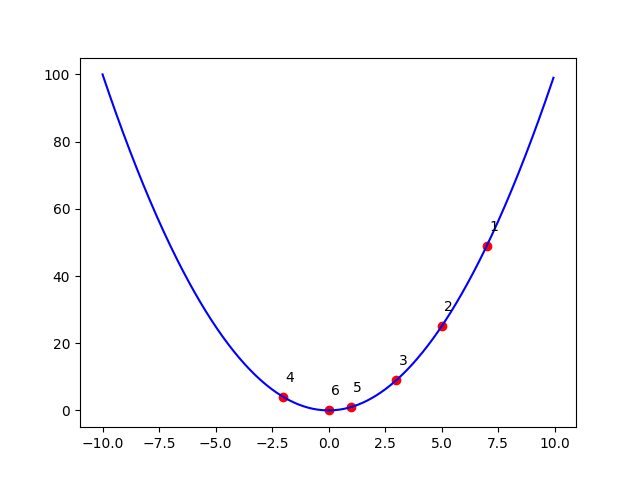
\includegraphics[scale=0.7]{imagenes/sgd.png}
		\caption{Oscilación alrededor del mínimo.}
		\label{img:oscilacion-sgd}
	\end{figure}

	En esta figura podemos ver cómo se produce una oscilación alrededor del mínimo. En funciones más complejas esta oscilación puede ser aún mayor y condicionar el funcionamiento del algoritmo de optimización. Esta variante del algoritmo hace que este zigzagueo u oscilación sea más leve, veamos el algoritmo en pseudocódigo:
	
	\begin{algorithm}[H]{\Large{\textbf{Gradiente Descendente Estocástico con momento}}}
		
		\vspace{15px}
		
		\caption{Gradiente Descendente Estocástico con momento}
		\label{alg:sgd-momento}
		\KwIn{Tasa de Aprendizaje $\epsilon$}
		\KwIn{Parámetros iniciales $\theta$}
		\KwIn{Tamaño de los lotes de datos $m$}
		\KwIn{Momento $\alpha$}
		\KwIn{Velocidad inicial $v$}
		
		\vspace{10px}
		
		\While{no se cumpla el criterio de parada}{
			
			Escoger un batch de datos de tamaño $m$ $x^{(1)}, ..., x^{(m)}$ con correspondientes objetivos $y^{(1)}, ..., y^{(m)}$
			
			Calculamos una estimación del gradiente.
			
			$\hat{g} \leftarrow \frac{1}{m}\nabla \sum_{i} L(f(x^{(i)};\theta), y^{(i)})$
			
			Actualizamos la velocidad.
			
			$v\leftarrow \alpha v - \epsilon \hat{g}$
			
			Actualizamos los parámetros.
			
			$\theta \leftarrow \theta + v$
			
		}
		
		\vspace{10px}
		
		\KwOut{Nuevos parámetros $\theta$}
		
		\vspace{5px}
	\end{algorithm}

	\item AdaGrad: esta es una versión adaptativa de SGD. El algoritmo varía los parámetros de forma inversamente proporcional a la raíz cuadrada de la suma de los cuadrados de los valores anteriores. Es decir, actualiza la tasa de aprendizaje decrementándola más rápido cuanto mayores sean las derivadas parciales. Como consecuencia de esto el avance en el espacio es más rápido que SGD. Veamos el pseudocódigo:
	
	\begin{algorithm}[H]{\Large{\textbf{Adagrad}}}
		
		\vspace{15px}
		
		\caption{Adagrad}
		\label{alg:adagrad}
		\textbf{Notación:} $\odot$ nota el producto componente a componente, $\sqrt{\cdot}$ es la raíz cuadrada componente a componente y las divisiones correspondientes son componente a componente.
		
		\KwIn{Tasa de Aprendizaje $\epsilon$}
		\KwIn{Parámetros iniciales $\theta$}
		\KwIn{Tamaño de los lotes de datos $m$}
		\KwIn{Constante inicial $\delta$ pequeña}
		
		\vspace{10px}
		
		$r\leftarrow 0$
		
		\While{no se cumlpa el criterio de parada}{
		
			Escoger un batch de datos de tamaño $m$ $x^{(1)}, ..., x^{(m)}$ con correspondientes objetivos $y^{(1)}, ..., y^{(m)}$
			
			Calculamos una estimación del gradiente.
			
			$\hat{g} \leftarrow \frac{1}{m}\nabla \sum_{i} L(f(x^{(i)};\theta), y^{(i)})$
			
			$r\leftarrow r + \hat{g}\odot \hat{g}$
			
			$\Delta \theta \leftarrow - \frac{\epsilon}{\delta + \sqrt{r}} \odot \hat{g}$
			
			$\theta \leftarrow \theta + \Delta \theta$

		}
		
		\vspace{10px}
		
		\KwOut{Nuevos parámetros $\theta$}
		
		\vspace{5px}
	\end{algorithm}

	\item RMSProp: en vez de ir acumulando los gradientes se hace una media exponencial, lo que teóricamente mejor el comportamiento al minimizar funciones no convexas (aquellas idóneas para SGD).
	
	\begin{algorithm}[H]{\Large{\textbf{RMSProp}}}
		
		\vspace{15px}
		
		\caption{RMSProp}
		\label{alg:rmsprop}
		\textbf{Notación:} $\odot$ nota el producto componente a componente, $\sqrt{\cdot}$ es la raíz cuadrada componente a componente y las divisiones correspondientes son componente a componente.
		
		\KwIn{Tasa de Aprendizaje $\epsilon$}
		\KwIn{Parámetros iniciales $\theta$}
		\KwIn{Tamaño de los lotes de datos $m$}
		\KwIn{Constante inicial $\delta$ pequeña}
		\KwIn{Tasa de decaimiento $\rho$}
		
		\vspace{10px}
		
		$r\leftarrow 0$
		
		\While{no se cumlpa el criterio de parada}{
			
			Escoger un batch de datos de tamaño $m$ $x^{(1)}, ..., x^{(m)}$ con correspondientes objetivos $y^{(1)}, ..., y^{(m)}$
			
			Calculamos una estimación del gradiente.
			
			$\hat{g} \leftarrow \frac{1}{m}\nabla \sum_{i} L(f(x^{(i)};\theta), y^{(i)})$
			
			$r\leftarrow \rho r + (1-\rho)\hat{g}\odot \hat{g}$
			
			$\Delta \theta \leftarrow - \frac{\epsilon}{\delta + \sqrt{r}} \odot \hat{g}$
			
			$\theta \leftarrow \theta + \Delta \theta$
			
		}
		
		\vspace{10px}
		
		\KwOut{Nuevos parámetros $\theta$}
		
		\vspace{5px}
	\end{algorithm}

	\item Adam: es una modificación de RMSProp con momento. Veamos el pseudocódigo:
	
	\begin{algorithm}[H]{\Large{\textbf{RMSProp}}}
		
		\vspace{15px}
		
		\caption{RMSProp}
		\label{alg:rmsprop}
		\textbf{Notación:} $\odot$ nota el producto componente a componente, $\sqrt{\cdot}$ es la raíz cuadrada componente a componente y las divisiones correspondientes son componente a componente.
		
		\KwIn{Tasa de Aprendizaje $\epsilon$}
		\KwIn{Parámetros iniciales $\theta$}
		\KwIn{Tamaño de los lotes de datos $m$}
		\KwIn{Constante inicial $\delta$ pequeña}
		\KwIn{Tasas de decaimiento $\rho_1 , \rho_2 \in [0,1)$}
		
		\vspace{10px}
		
		$s\leftarrow 0$
		
		$r\leftarrow 0$
		
		$t\leftarrow 0$
		
		\While{no se cumlpa el criterio de parada}{
			
			Escoger un batch de datos de tamaño $m$ $x^{(1)}, ..., x^{(m)}$ con correspondientes objetivos $y^{(1)}, ..., y^{(m)}$
			
			Calculamos una estimación del gradiente.
			
			$\hat{g} \leftarrow \frac{1}{m}\nabla \sum_{i} L(f(x^{(i)};\theta), y^{(i)})$
			
			$t\leftarrow t+1$
			
			$s\leftarrow \rho_1 \cdot s + (1-\rho_1)\hat{g}$
			
			$r\leftarrow \rho_2 \cdot s + (1-\rho_2)\hat{g}\odot \hat{g}$
			
			$\hat{s}\leftarrow \frac{s}{1-\rho_1^r}$
			
			$\hat{r}\leftarrow \frac{r}{1-\rho_2^r}$
			
			$\Delta \theta \leftarrow - \frac{\epsilon}{\delta + \sqrt{\hat{r}}}\hat{s}$
			
			$\theta \leftarrow \theta + \Delta \theta$
			
		}
		
		\vspace{10px}
		
		\KwOut{Nuevos parámetros $\theta$}
		
		\vspace{5px}
	\end{algorithm}
\end{itemize}

Con esto ya hemos cubierto cómo aprende una red neuronal de forma completa.